\documentclass[UTF8]{ctexart}

\usepackage{WeeklyReport}
\usepackage{graphicx}
\usepackage{amsmath}
\usepackage{amssymb}

\title{周报06}
\author{Jeff\ Fu}
\date{\today}

\begin{document}
    \maketitle
    % \tableofcontents
    \section{学习内容}
        \begin{itemize}
            \item 阅读Feature Selection相关论文
        \end{itemize}
    \section{学习收获}
        这周看了 Concrete Autoencoders for Differentiable Feature Selection and Reconstruction (ICML2019) 这篇文章,
        整理一下文章的思路。
        \subsection{Concrete Autoencoders for Differentiable Feature Selection and Reconstruction}
            \subsubsection{基本思路}
                使用 Concrete Autoencoder 进行Feature Selection,导出一个最 informative 的 feature 子集,
                然后再训练一个神经网络根据被选出的 feature 进行 input 的重建。

                整个方法是 unsupervised 的,使用一个 concrete selector layer 作为 encoder,decoder 则采用常规的结构。
                使用 selected feature 进行重建可以减少很多计算量。文章的关注点在于:dataset 中有哪些 feature 是重要的,
                哪些 feature 是多余而不需要参与计算的(有点类似 PCA 中降维的概念)。
            \subsubsection{Concrete Selector Layer}
                Concrete Selector Layer 是基于 Concrete random variables 的,而 Concrete random variables 用于产生对 one-hot vector 的持续性 relaxation,
                relax 的程度由一个 temperature 参数 $T \in (0, \infty)$ 决定。

                产生 Concrete distribution 的公式如下:

                $$
                    \mathbf{m}_j = \frac{\exp((\log \mathbf{\alpha}_j + \mathbf{g}_j)/T)}{\sum_{k=1}^d \exp((\log \mathbf{\alpha}_k + \mathbf{g}_k)/T)}
                $$

                其中 $\alpha \in \mathbb{R}^d_{>0}$ 是一个参数向量,Grumble 分布的样本,$\mathbf{m}_j$ 表示的是某个样本向量中的第 $j$ 个元素。
                在 $T \rightarrow 0$ 时,Concrete Distribution 收敛到 Discrete Distribution(以 $\alpha_j / \sum_p \alpha_p$ 的概率让 $\mathbf{m}_j = 1$ )。

                利用 Concrete Distribution,按照如下方式选取 feature:对于 Concrete Selector Layer 中的每一个结点,
                生成一个 $d$ 维的 Concrete random variable $\mathbf{m}^{(i)}, i \in \{1 \dots k\}$ ,
                则对于 concrete selector layer 的第 $i$ 个结点 $u^{(i)}$ ,其输出为 $\mathbf{x}\cdot \mathbf{m}^{(i)}$。

                \begin{figure}[ht]
                    \centering
                    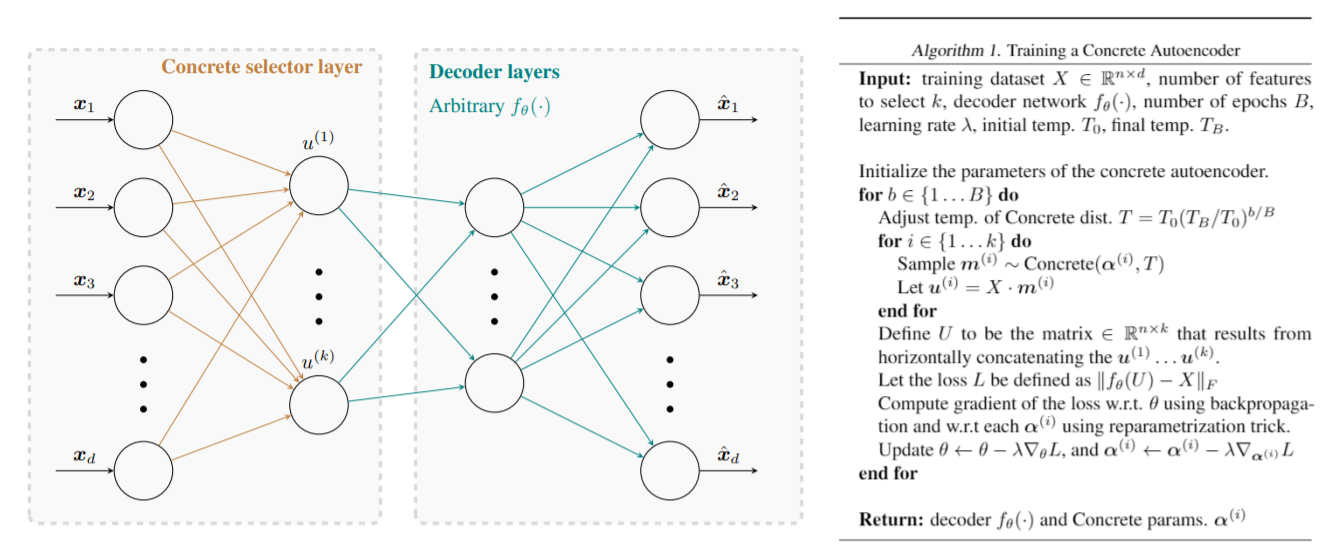
\includegraphics[scale=0.36]{Week06_concrete.png}
                    \caption{Concrete Selector Layer结构及训练算法}
                    \label{fig:concrete}
                \end{figure}

                按我的理解,上述过程实际上只是做了一个线性组合,跟一层 FC 的功能类似,但是当 $T \rightarrow 0$ 时,
                concrete selector layer 只会输出 input feature 中的一个,而在整个训练过程中,$T$ 是逐渐减小的,
                因此可以认为这个 concrete selector layer 在训练过程中进行的是从 FC 向 discrete distribution 的过渡。
                训练完成后,在测试过程中,把 concrete selector layer 换成 discrete $\arg \max$ layer,
                此时第 $i$ 个神经元的输出为 $\mathbf{x}_{\arg \max_j \alpha_j^{(i)}}$ 。

                对于参数向量 $\alpha$ ,随机初始化成较小的正值,使得 selector layer 能够随机地(stochastic)寻找 input feature 的
                不同线性组合,随着网络的训练,$\alpha$ 逐渐变得稀疏,即网络越来越认为某些特定 feature 是重要的。

                Concrete Selector Layer 的结构和训练算法如图 \ref{fig:concrete} 所示。
            \subsubsection{Annealing Schedule}
                (看名字感觉上是借用物理学中的温度传递和衰退公式)

                从前面的公式可以看出,temperature $T$ 对于网络结点的输出有显著影响,当 $T$ 较大时,
                网络输出的是 input feature 的线性组合,反过来,当 $T$ 很小时,网络的输出就变得离散化,
                可见无论 $T$ 取哪一个固定值,都不能很好地筛选出合适的 feature,因此 $T$ 需要在训练过程中进行变化。

                论文中提出了一个退火过程公式,用于在每个 epoch 更新 $T$ 的值,假设初始状态为 $T_0$ ,
                最终衰减到的状态为 $T_B$ ,则每个 epoch 中的 $T$ 的值为:

                $$
                    T(b) = T_0(\frac{T_B}{T_0})^{\frac{b}{B}}
                $$

                其中 $b$ 和 $B$ 分别表示当前训练的 epoch 和总的训练 epoch。

                前面的 concrete random variable 可能很难用在 MSDA 的问题中,但是这个退火的想法感觉会有效,
                退火是 $T$ 的一个更新策略,而这个更新策略使得在训练结束后,所得到的结果是离散的,这才算是真正意义上地对 feature 进行了选择,
                之前我实现 PAL 使用的是 regularization 的方法,实际上最终结果是否离散无法确定。
            \subsubsection{小结}
                这篇文章中的 feature selection 是在 reconstruction 层面上选取合适的 feature,而在 MSDA 的问题中,
                需要选取不同 Source 之间相互“接近”的 feature,所选出的 feature 未必是 source 中最显著的 feature,
                与这篇文章的主要思想略有不同。但是文中的一些技巧可以借用,比如最终要保证 sparsity,选择出来的 feature 在各自的 source 中尽量显著。
    \section{启发}
        \begin{enumerate}
            \item 也许可以用 concrete selector layer 的方式选取 multi-source 的特征,但原文的思路实际上是类似 PCA 中降维的思想,
                而在 MSDA 的问题中,目的不在于降维,而是筛选出不同 source 之间共通的 feature,这样考虑的话,
                传统的 feature selection 方法并不一定适用(而生成 concrete random variable 的那一部分感觉可以挪过来试一试)
            \item 退火的公式让人眼前一亮,在 PAL 的设计中,我也是希望选取一些 feature 而不是得到线性组合,即需要保持 sparsity,
                如果使用文中的退火公式,也许可以让 PAL 的训练更符合预期(原本的想法是使用较强的 regularization,但这样感觉上会限制 PAL 本身的作用)
            \item 在选取不同 source 之间的公共 feature 时,还需要尽可能保证所选 feature 能包含 source 的大部分信息
                (在 reconstruction 的任务中可能比较看重这个,但在 MSDA 中是否适用还不确定)
        \end{enumerate}
    \section{疑问/困难}
        \begin{enumerate}
            \item 从目前看到的 feature selection 的文章看来,其目标在于降维而不是根据不同的 source domain 找到通用的 feature,
                如果在单源情况也许会有效果(指通过减少 feature 数量而提高性能),但感觉上很难体现出多源的特性
            \item 应该如何将 NN 与退火过程结合起来,既保留 NN 的广度,又使得最终的结果是 sparse 的
            \item 按我的想法,MSDA 中选出来的特征,应当是由各个源域共同决定的,而这个特征并不一定能包含源的大部分信息,甚至某些情况下只包含少部分信息,
                这样去想的话,也许并不需要去关心 reconstruction loss
        \end{enumerate}
\end{document}
